% !TeX spellcheck = en_GB

\documentclass[aspectratio=169,]{beamer}

\usepackage[utf8]{inputenc}
\usepackage[english]{babel}
%\usepackage{appendixnumberbeamer}

\usepackage{tikz}
\usetikzlibrary{shapes,arrows,positioning,calc}

\tikzstyle{startstop} = [ellipse, draw, fill=bg, text=structure, text width=3em, text badly centered, inner sep=0pt]
\tikzstyle{block} = [rectangle, draw, fill=bg, text=structure, text width=5em, text centered]
\tikzstyle{decision} = [diamond, aspect=3, draw, fill=bg, text=structure, text width=3em, text badly centered, inner sep=0pt]
\tikzstyle{input} = [trapezium, draw, fill=bg, text=structure, text width=5em, text centered, trapezium right angle=120]
\tikzstyle{output} = [trapezium, draw, fill=bg, text=structure, text width=5em, text centered, trapezium right angle=120]

\tikzstyle{line} = [draw, -latex']

%\usepackage{xcolor}
\usepackage{listings}

\lstdefinestyle{pseudo}{
	backgroundcolor=\color{bg},
	keywordstyle=\color{alert},
	numberstyle=\tiny\color{fg!50},
	numbers=left,
	%commentstyle=\color{mGreen},
	%stringstyle=\color{mPurple},
    mathescape=true,
	basicstyle=\scriptsize,
    keywords={input,output,begin,end,if,then,else,while,do,for,each,return}
	%tabsize=4,
	%breakatwhitespace=false,
	%breaklines=true,
	%captionpos=b,
	%keepspaces=true,
	%numbersep=5pt,
	%showspaces=false,
	%showstringspaces=false,
	%showtabs=false,
	%language=C
}

\usepackage{minted}


\usetheme[titleformat=smallcaps, numbering=fraction, background=light, progressbar=frametitle]{metropolis}

\title{Digital Technology}
\subtitle{Final recap: the k-means algorithm}

\author{Stefano Cereda\\
stefano.cereda@polimi.it
}
\date{28/05/2020}
\institute[PoliMi]{Politecnico Milano}
\logo{
\includegraphics[width=15mm]{../logopolimi}}

\setbeamercovered{invisible}

\makeindex

\begin{document}
\begin{frame}
    \maketitle
\end{frame}

\begin{frame}[fragile]{Exercise 1 --- Loading datasets}
    The following code allows you to get a list of files in the current directory:
    \begin{minted}[autogobble]{Python}
        import os
        file_list = os.listdir()
    \end{minted}

    You can get the content of another directory by specifying the path as an argument:
    \begin{minted}[autogobble]{Python}
        import os
        file_list = os.listdir('./dataset/')
    \end{minted}

    Use the code to open all the csv files of the stock market dataset, creating a dictionary that links each company
    name to its dataframe.

    \pause
    Sometimes, the code will generate an error.
\end{frame}

\begin{frame}[fragile]{Try/except}
    The previous exercise generates an error because some of the files are empty and pandas cannot load them.
    If you want to handle these errors you can use the \emph{try/except} statements.

    \begin{itemize}
        \item The \emph{try} block lets you test a block of code for errors
        \item The \emph{except} block lets you handle the error
    \end{itemize}

    \begin{minted}[autogobble]{Python}
        try:
            print(x)
        except:
            print("An error occurred")
    \end{minted}
    The print instruction will generate an error, since $x$ in not defined. Instead of terminating the execution, Python
    will execute the \emph{except} block, going on with the program.
\end{frame}

\begin{frame}{Try/except}
    Use the try/except statement and the \emph{continue} statement (which allows you to go to the next iteration of a loop) to fix
    the previous exercise.
\end{frame}

\begin{frame}{Exercise 2 --- Generating ROI lists}
    Write a function that:
    \begin{itemize}
        \item receives the loaded dataset
        \item for each company, runs a simulation of the two trading strategies we defined in previous classes
            (keep\_strategy and gain\_strategy)
        \item returns two lists containing the ROIs of the two strategies.
    \end{itemize}
\end{frame}

\begin{frame}{Exercise 3 --- Scatter plot of the ROIs}
    Produce a scatter plot of the two ROI lists.

    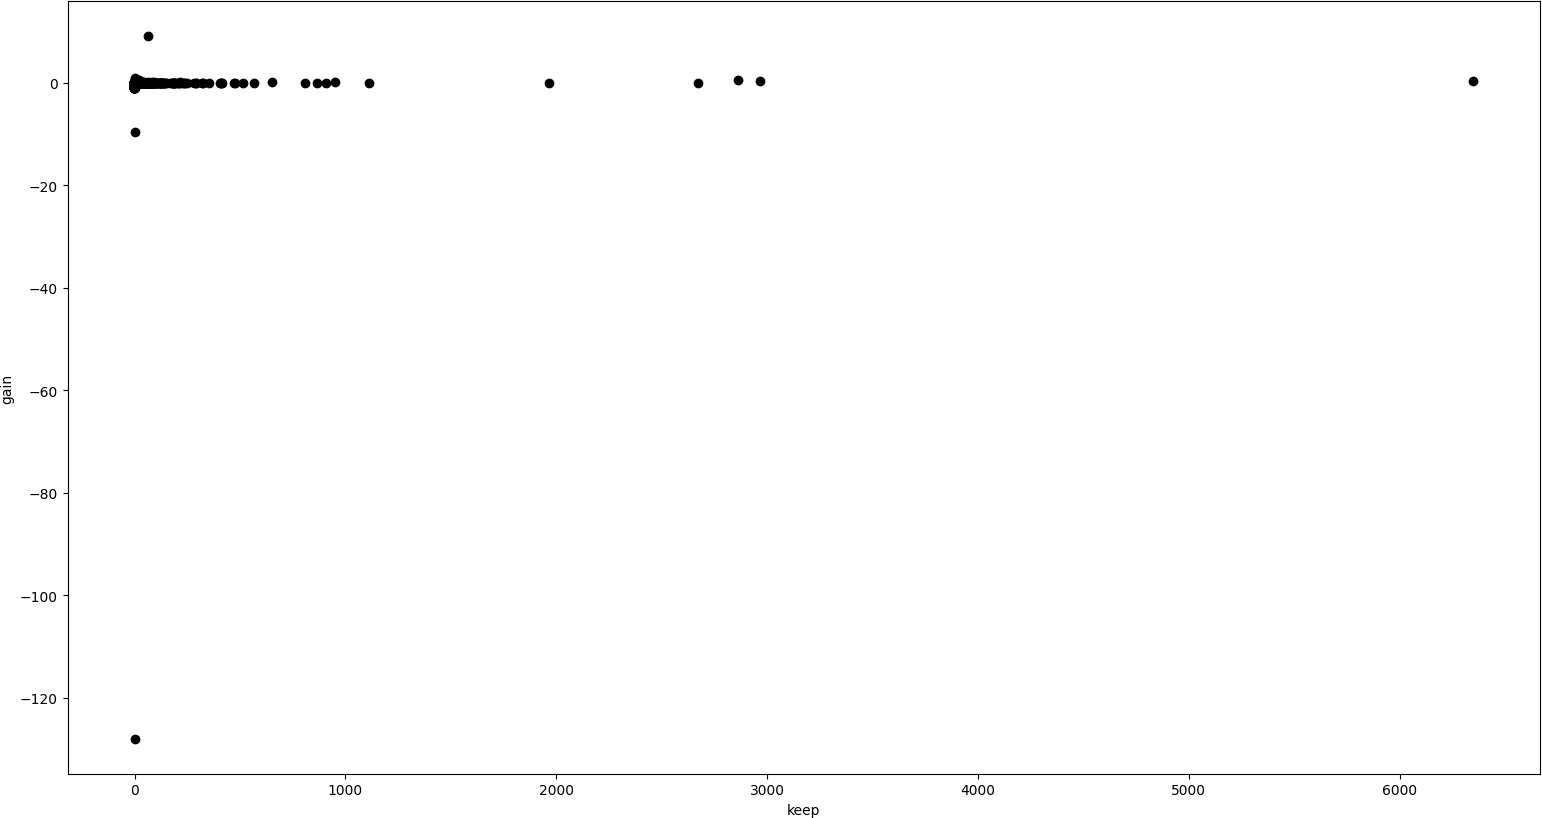
\includegraphics[width=0.8\textwidth]{./scatterplot.png}
\end{frame}

\begin{frame}{K-means clustering}
    K-means is a clustering algorithm that partitions $n$ observations into $k$ clusters.

    It is composed by 3 steps:
    \begin{enumerate}
        \item Initialisation: $k$ initial centroids are generated at random
        \item Assignment: each observation is assigned to the cluster with the nearest centroid
        \item Update: recompute the centroids as the mean of the assigned points
    \end{enumerate}

    Assignment and Update are repeated iteratively until the assignments no longer change.
\end{frame}

\begin{frame}{Exercise 3 --- K-means initialisation}
    Generate $k=4$ centroids for the ROI points and represent them on the scatter plot.
    Save the centroids in a dictionary linking each centroid to its coordinates.

    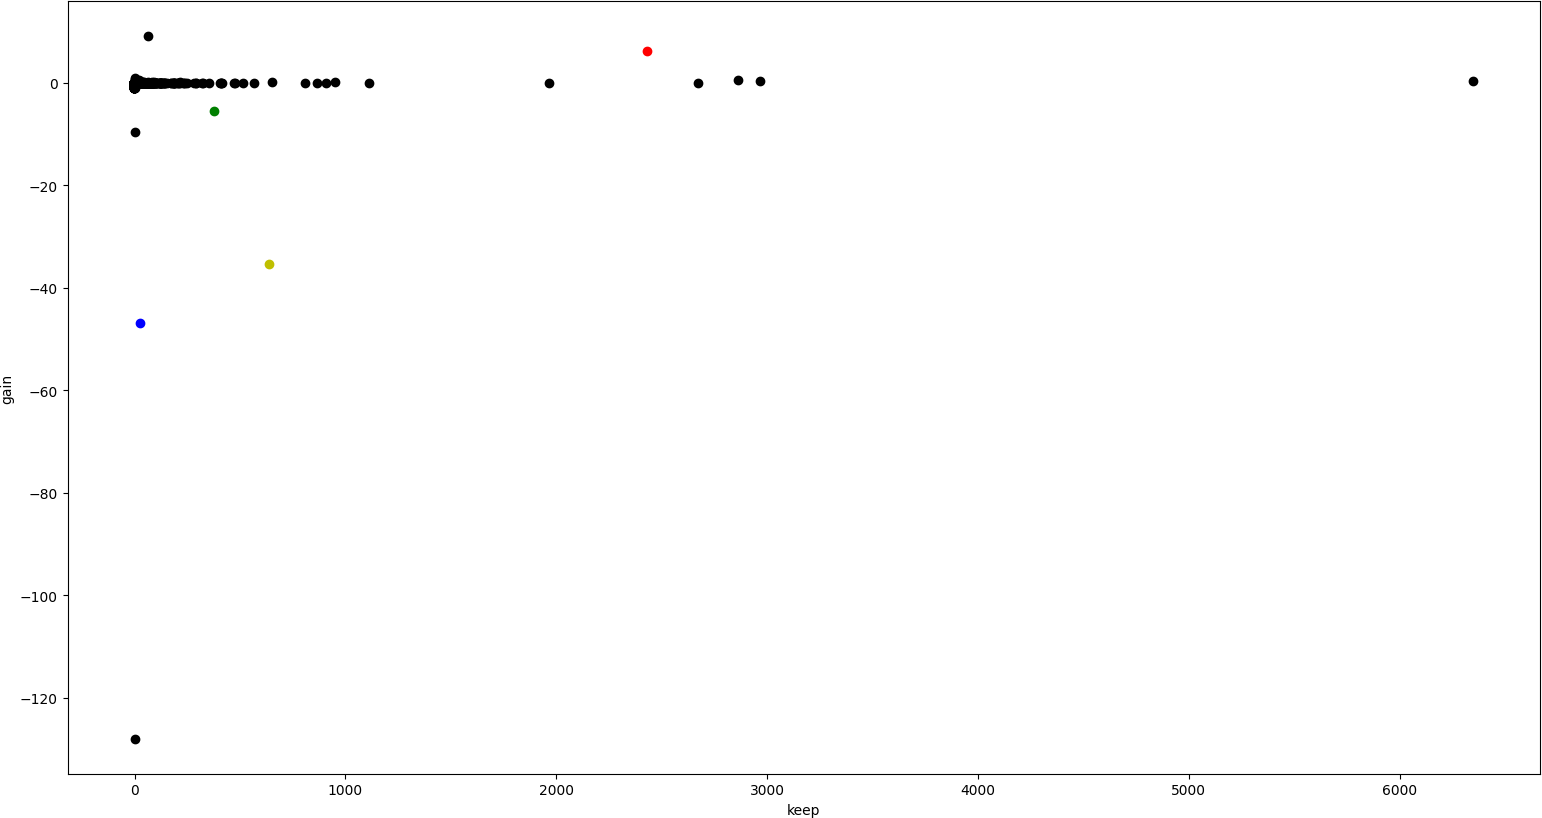
\includegraphics[width=0.8\textwidth]{./kmeans-init.png}
\end{frame}

\begin{frame}[fragile]{The zip function}
    The \emph{zip} function creates an iterator that aggregate elements from two or more iterables:
    \begin{minted}[autogobble]{Python}
        l1 = [1,2,3,4]
        l2 = ['a', 'b', 'c', 'd']
        for thing in zip(l1, l2):
            print(thing)
    \end{minted}
    \begin{minted}[autogobble]{Text}
        (1, 'a')
        (2, 'b')
        (3, 'c')
        (4, 'd')
    \end{minted}

    Use the zip function to create a list of (x, y) couples representing the position of each ROI point in the scatter plot.
\end{frame}


\begin{frame}{Exercise 5 --- K-means assignment}
    Write a python function that receives the list of points as computed in the previous exercise, the centroids
    dictionary and produces a list containing the closest centroid to each cluster.

    You can compute the euclidean norm of a vector $v$ using \emph{numpy.linalg.norm(v)}.

    Create a scatter plot representing the cluster of each point.

    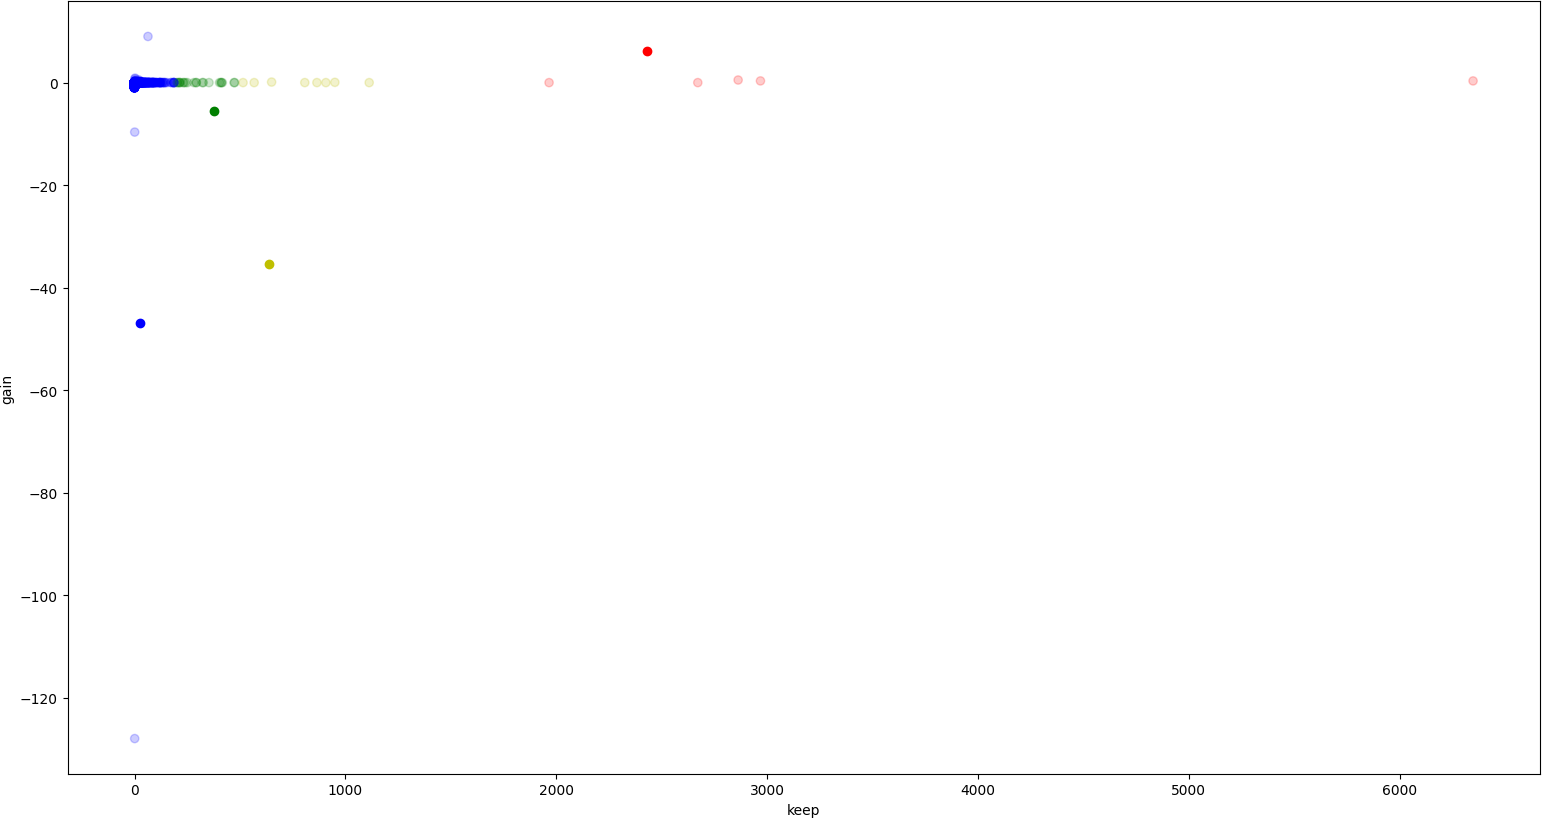
\includegraphics[width=0.5\textwidth]{./kmeans-assign.png}
\end{frame}

\begin{frame}{Exercise 6 --- K-means update}
    Write a function that receives a list of points and a list of assignments and computes the new positions of the
    centroids. Update the plot.

    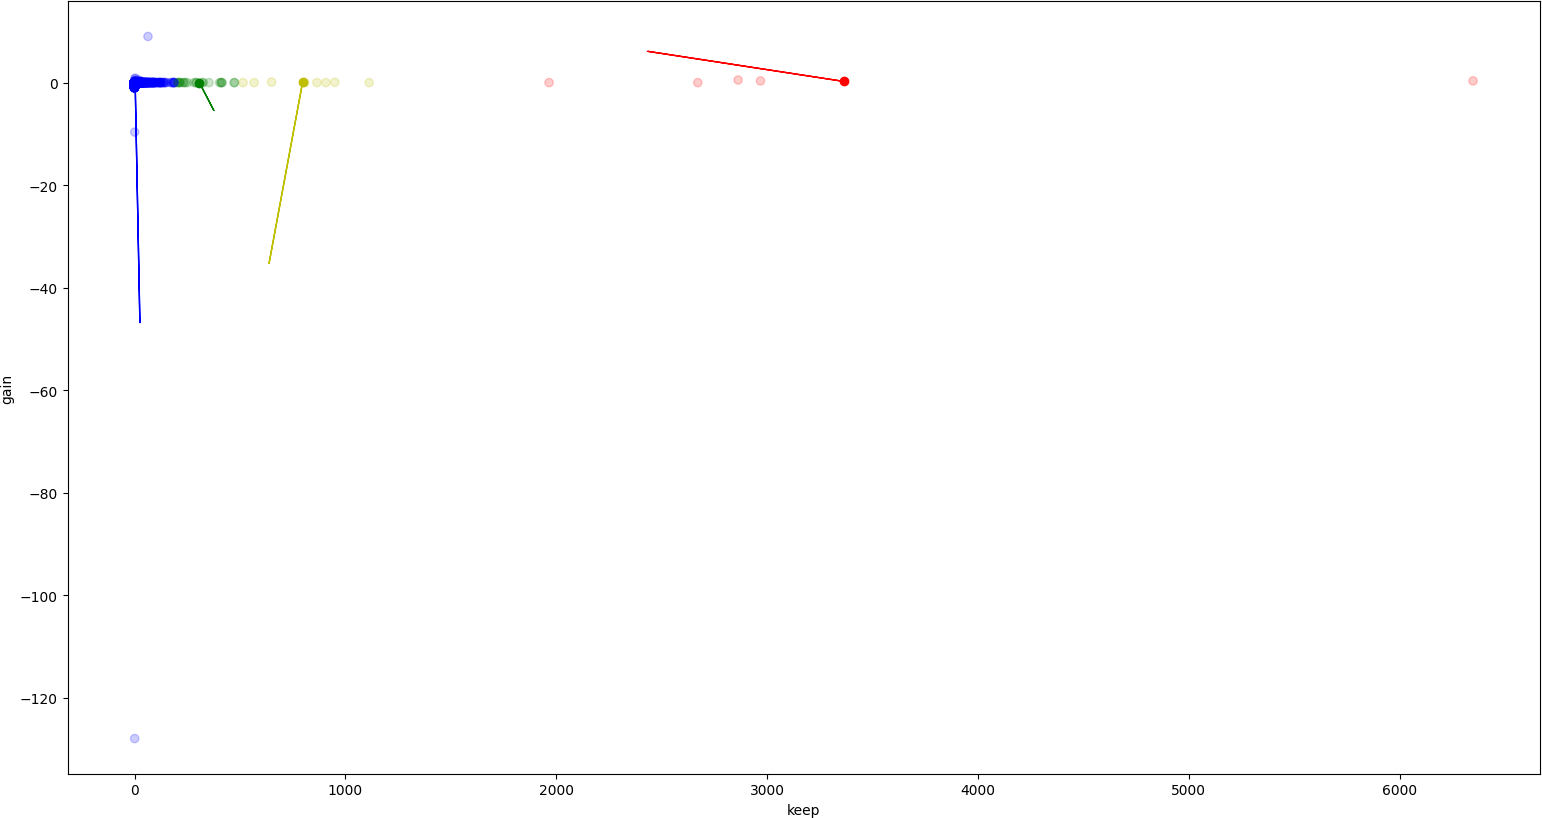
\includegraphics[width=0.8\textwidth]{./kmeans-update.png}
\end{frame}

\begin{frame}{Exercise 7 --- K-means loop}
    Repeat steps 2 and 3 of the k-means algorithm until convergence.

    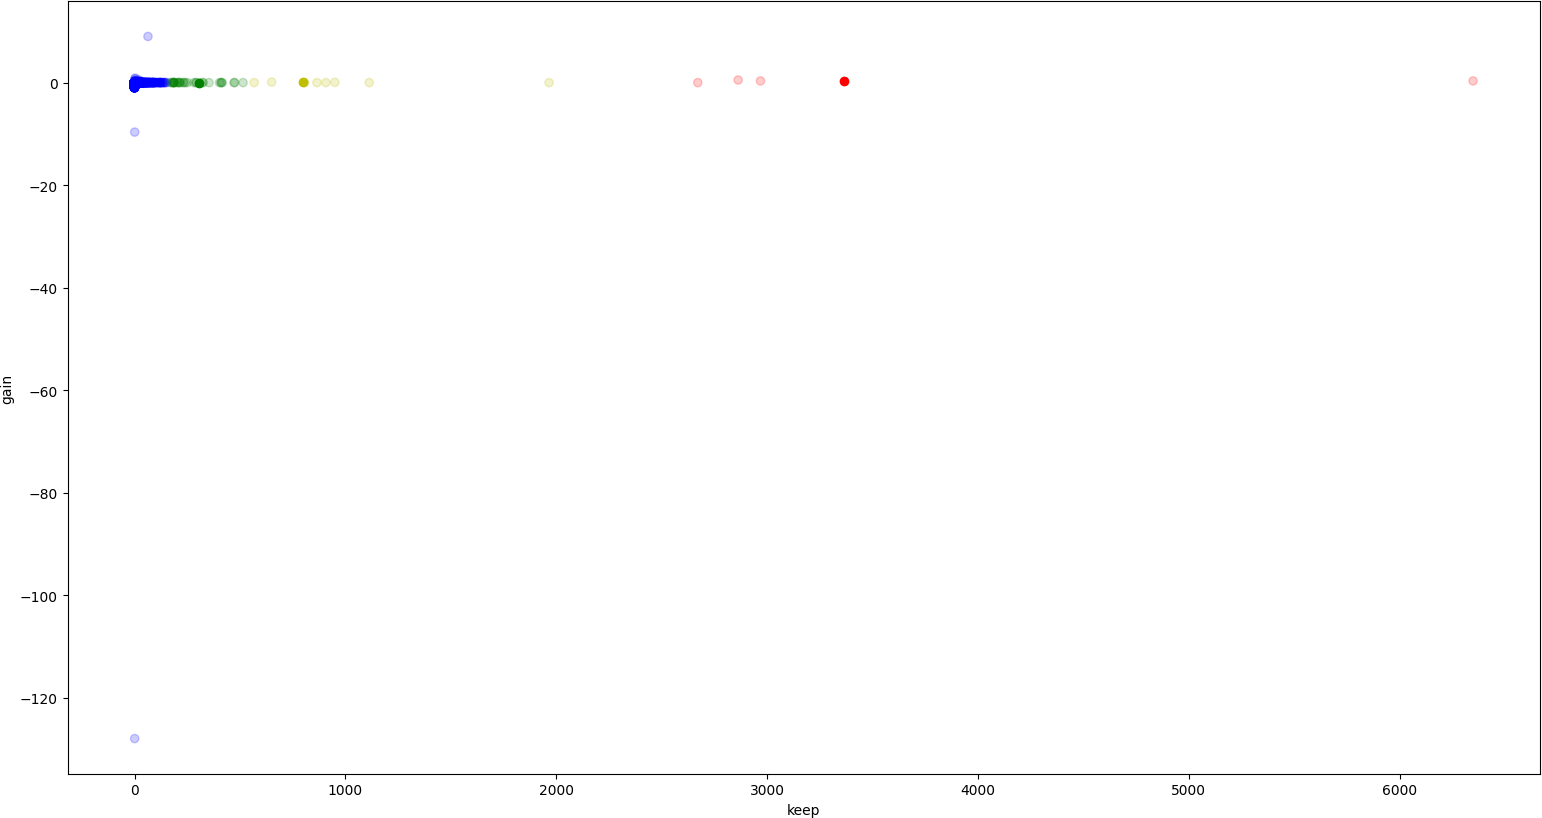
\includegraphics[width=0.4\textwidth]{./kmeans-loop1.png}
    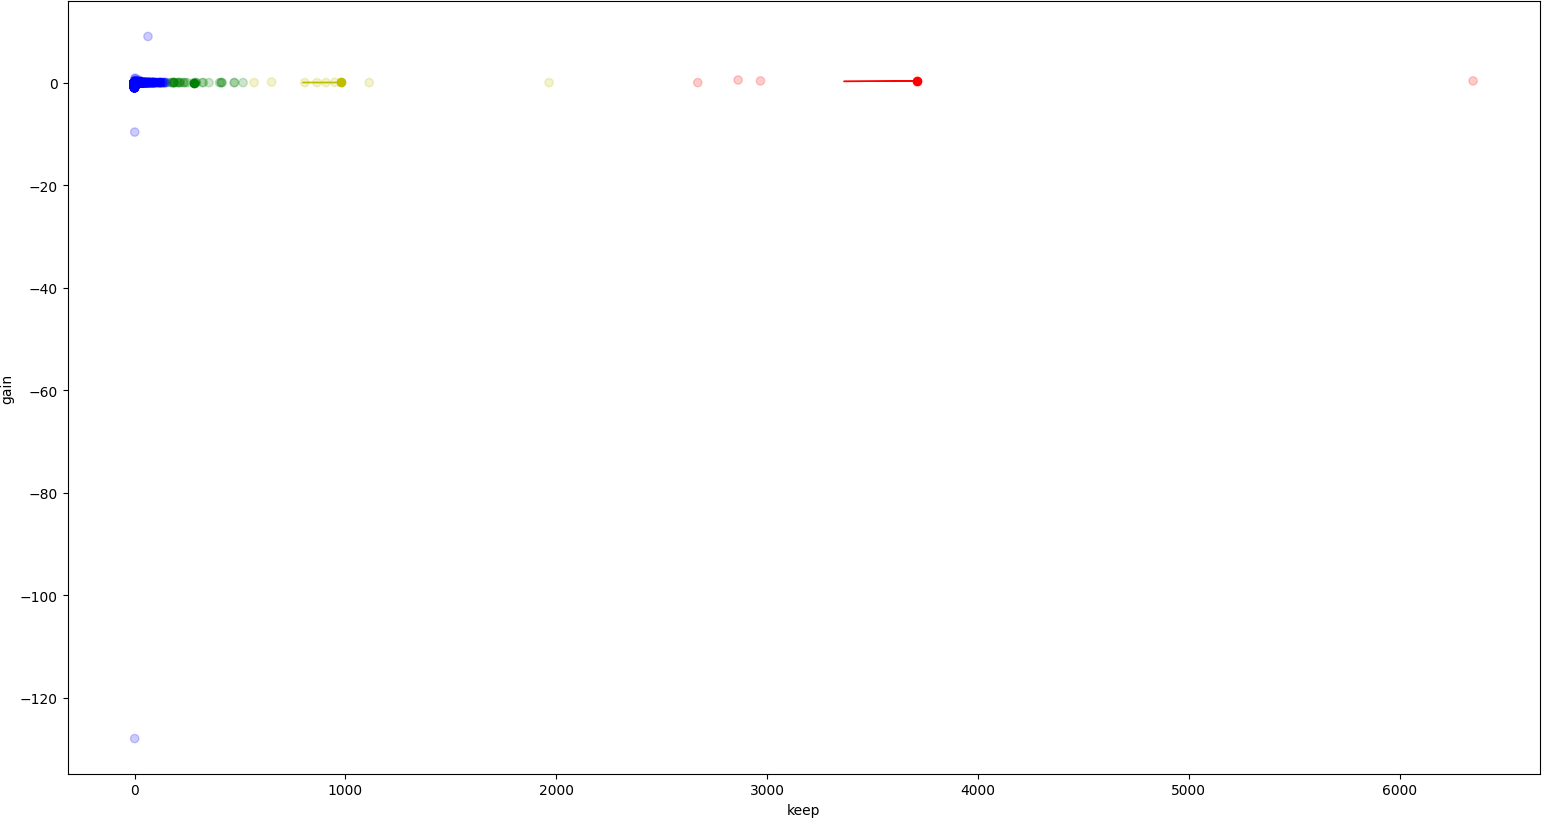
\includegraphics[width=0.4\textwidth]{./kmeans-loop2.png}

    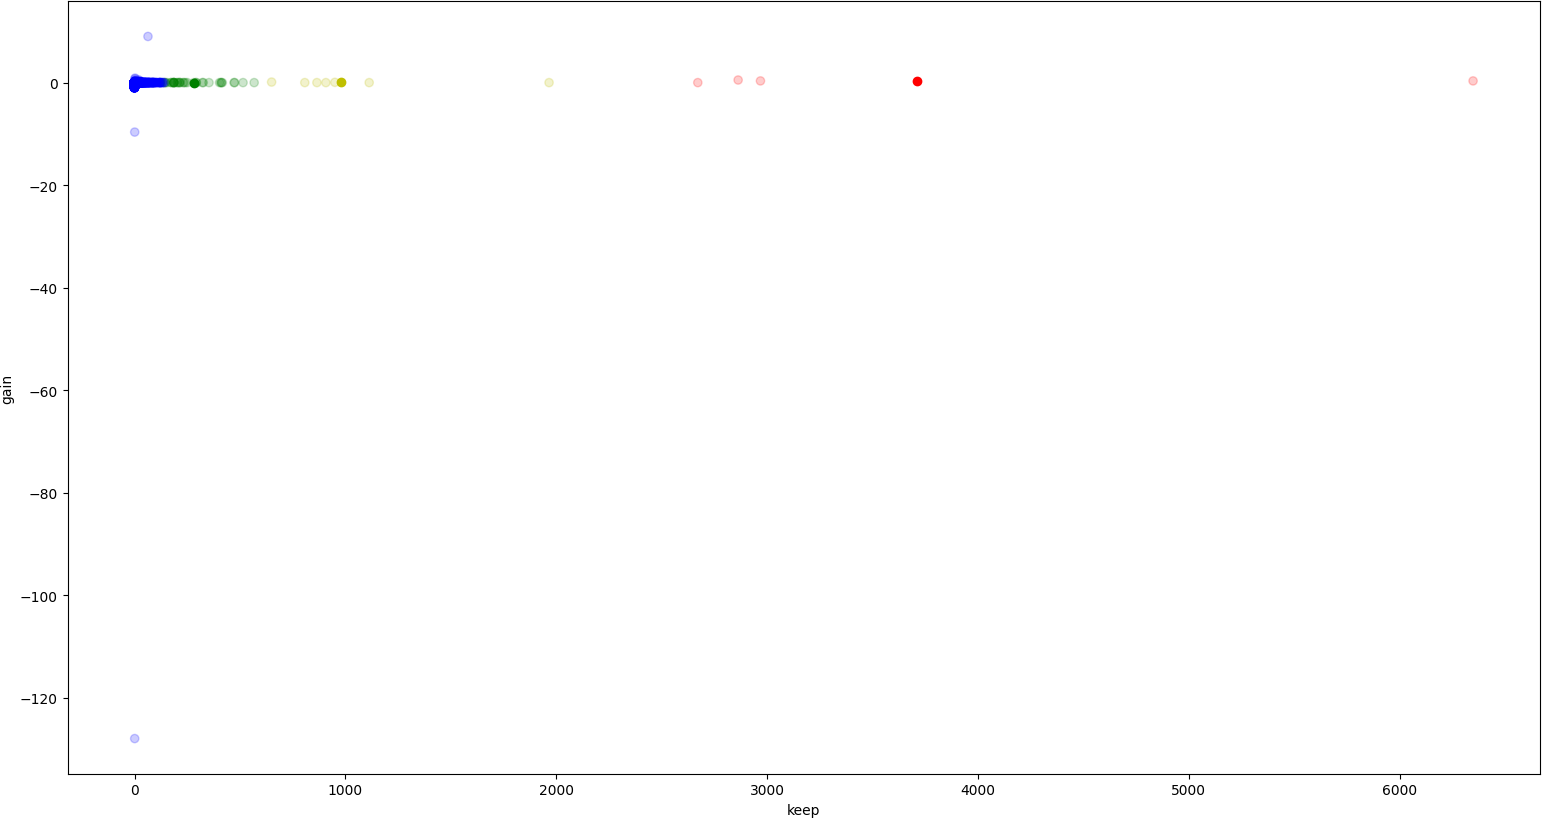
\includegraphics[width=0.4\textwidth]{./kmeans-loop3.png}
    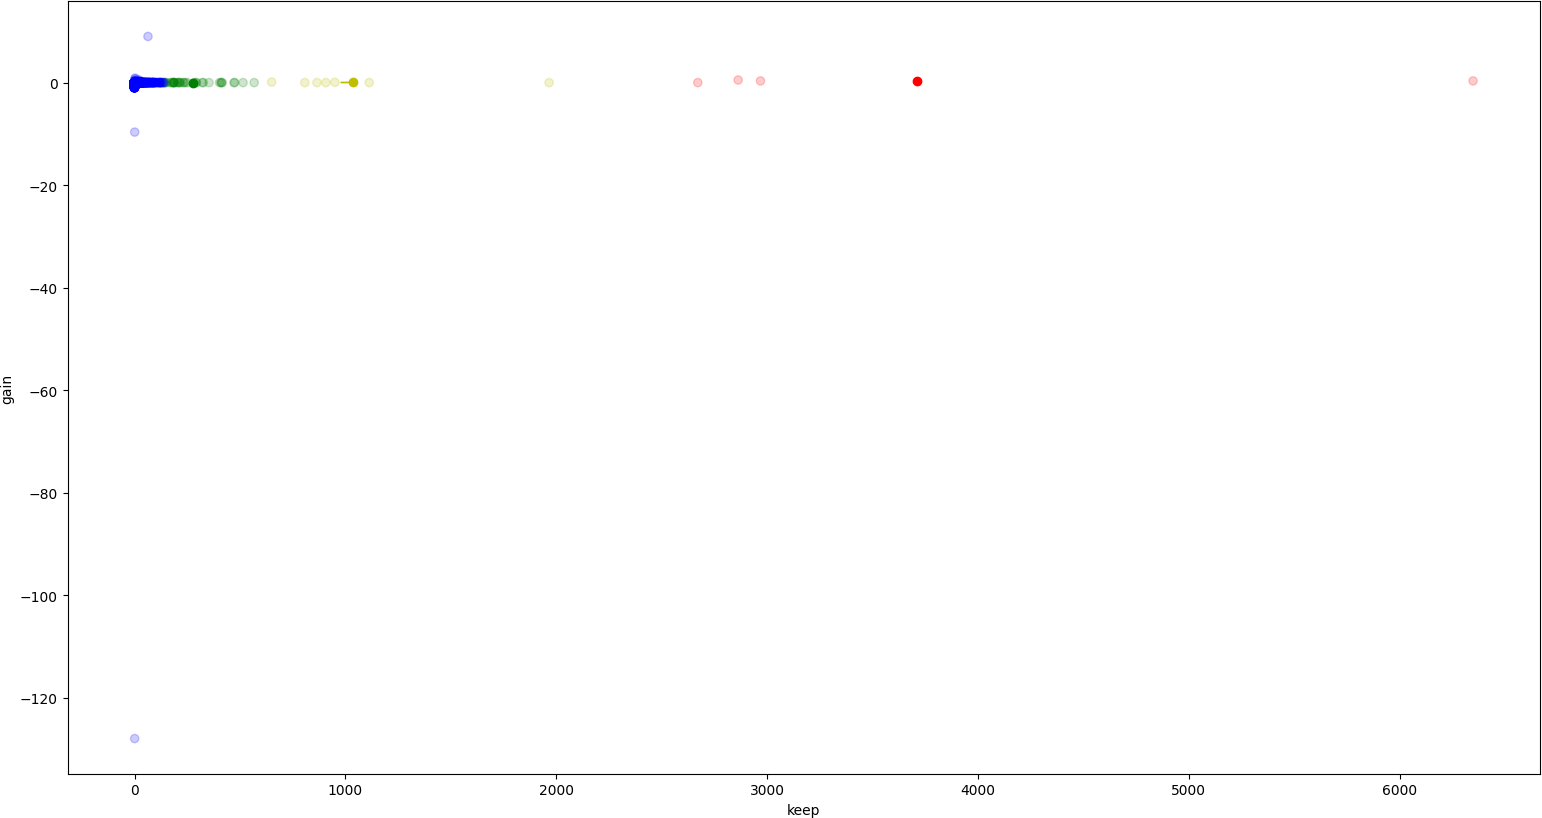
\includegraphics[width=0.4\textwidth]{./kmeans-loop4.png}
\end{frame}

\end{document}
